% % % % % % % part-02% % % % % % % % % %
\documentclass[12pt]{article}

\usepackage{tikz}

\author{BKP}
\title{Drawing in \LaTeX\ Using PGF/TikZ}\date{}

\begin{document}
	\maketitle\vskip-25pt\hrule\vskip10pt

%\begin{tikzpicture}[option]
%<tikz codes>
%\end{tikzpicture}

%\tikz[options]{<tikz codes>}

%\begin{tikzpicture}[option]
%\path[option1][option2] <specification> ;
%\end{tikzpicture}

\begin{tikzpicture}
\draw (0,0)--(15mm,0) ;
\end{tikzpicture}

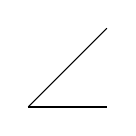
\begin{tikzpicture}
\draw (0,0)--(1,0) ;
\draw (0,0)--(1,1) ;
\end{tikzpicture}

\vskip25pt
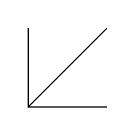
\begin{tikzpicture}
\draw (1,0)--(0,0)--(0,1) (0,0)--(1,1) ;
\end{tikzpicture}

\vskip25pt
\begin{tikzpicture}
%\draw (0,0)--(1,0)--(1,1) (0,1)--(0,0) ;
\draw (0,0) rectangle (1,3);
\draw (3,0)--(4,0) -- (4,4)--cycle;
\end{tikzpicture}

\vskip25pt
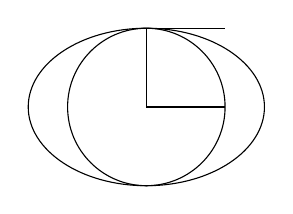
\begin{tikzpicture}
\draw (0,0) circle [radius=1cm];
\draw (0,0) circle [x radius=1.5cm, y radius= 1cm];
\draw (1,0)--(0,0)--(0,1) parabola (1,1)  ;
\end{tikzpicture}

\end{document}
